\subsection{Danh sách Use Case}

\begin{table}[H]
\centering
\small
\caption{Danh sách Use Case của hệ thống}
\label{tab:ch2-3}
\begin{tabularx}{\textwidth}{|>{\raggedright\arraybackslash}p{0.18\textwidth}|>{\raggedright\arraybackslash}X|>{\raggedright\arraybackslash}p{0.22\textwidth}|>{\raggedright\arraybackslash}p{0.18\textwidth}|}
\hline
\textbf{Mã} & \textbf{Tên Use Case} & \textbf{Tác nhân} & \textbf{Người phụ trách} \\
\hline
UC01 & Tạo phòng và giường & Cán bộ & Tùng \\
\hline
UC02 & Tìm phòng còn chỗ phù hợp & Sinh viên & Tùng \\
\hline
UC03 & Gửi yêu cầu đặt phòng & Sinh viên & Nhân \\
\hline
UC04 & Giữ phòng và giường cho sinh viên & Cán bộ & Nhân \\
\hline
UC05 & Lập hợp đồng thuê phòng cho sinh viên & Cán bộ & Huân \\
\hline
UC06 & Xác nhận bàn giao phòng cho sinh viên & Cán bộ & Huân \\
\hline
UC07 & Phát hành khoản phí nội trú theo kỳ & Cán bộ & Tuấn \\
\hline
UC08 & Thanh toán khoản phí nội trú & Sinh viên & Tuấn \\
\hline
UC09 & Gửi yêu cầu trả phòng & Sinh viên & Dũng \\
\hline
UC10 & Xác nhận hoàn tất trả phòng & Cán bộ & Dũng \\
\hline
\end{tabularx}
\end{table}

\subsection{Ma trận tác nhân – Use Case}

\begin{table}[H]
\centering
\small
\caption{Ma trận tác nhân -- Use Case}
\label{tab:ch2-4}
\begin{tabularx}{\textwidth}{|>{\raggedright\arraybackslash}X|>{\centering\arraybackslash}p{0.22\textwidth}|>{\centering\arraybackslash}p{0.22\textwidth}|}
\hline
\textbf{Use Case} & \textbf{Sinh viên} & \textbf{Cán bộ} \\
\hline
UC01 Tạo phòng và giường &  & X \\
\hline
UC02 Tìm phòng còn chỗ phù hợp & X & \\
\hline
UC03 Gửi yêu cầu đặt phòng & X & \\
\hline
UC04 Giữ phòng và giường cho sinh viên &  & X \\
\hline
UC05 Lập hợp đồng thuê phòng &  & X \\
\hline
UC06 Xác nhận bàn giao phòng &  & X \\
\hline
UC07 Phát hành khoản phí nội trú theo kỳ &  & X \\
\hline
UC08 Thanh toán khoản phí nội trú & X & \\
\hline
UC09 Gửi yêu cầu trả phòng & X & \\
\hline
UC10 Xác nhận hoàn tất trả phòng &  & X \\
\hline
\end{tabularx}
\end{table}

\subsection{Biểu đồ Use Case tổng quát}


\subsection{Biểu đồ Use Case phân rã theo chức năng}


\section{Phân tích nhóm chức năng xem phòng}

Nhóm chức năng xem phòng của \textbf{Hệ thống quản lý ký túc xá PTIT} bao gồm hai chức năng: cán bộ tạo phòng và giường, sinh viên tìm phòng còn chỗ phù hợp. UC01 tạo lập dữ liệu phòng, giường và trạng thái khả dụng ban đầu. UC02 khai thác dữ liệu đó để cung cấp cho sinh viên danh sách phòng phù hợp và còn ít nhất một giường trống.

\subsection{UC01 Cán bộ tạo phòng và giường}

\subsubsection{Mục đích và mô tả chức năng}

UC01 cho phép cán bộ quản lý ký túc xá tạo mới một phòng thuộc tòa nhà đã có trong hệ thống, đồng thời tạo danh sách các giường thuộc phòng đó.

Cán bộ nhập thông tin phòng gồm mã phòng, tên phòng, loại phòng, giới tính sử dụng, sức chứa, mức phí nội trú hằng tháng và danh sách mã giường. Hệ thống kiểm tra tính hợp lệ của dữ liệu trước khi lưu phòng cùng toàn bộ danh sách giường.

\subsubsection{Tác nhân, tiền điều kiện và hậu điều kiện}


\subsubsection{Luồng sự kiện chính}


\subsubsection{Luồng thay thế và ngoại lệ}


\subsubsection{Quy tắc nghiệp vụ và dữ liệu liên quan}


\subsubsection{Sơ đồ lớp UC01}


\subsection{UC02 Sinh viên tìm phòng còn chỗ phù hợp}

\subsubsection{Mục đích và mô tả chức năng}


\subsubsection{Tác nhân, tiền điều kiện và hậu điều kiện}


\subsubsection{Luồng sự kiện chính}


\subsubsection{Luồng thay thế và ngoại lệ}


\subsubsection{Quy tắc nghiệp vụ và dữ liệu liên quan}


\subsubsection{Sơ đồ lớp UC02}


\subsection{Quan hệ nghiệp vụ giữa UC01 và UC02}


\section{Phân tích nhóm chức năng đặt phòng}

\subsection{UC03 Sinh viên gửi yêu cầu đặt phòng}

\subsubsection{Mục đích và mô tả chức năng}

\paragraph{Mục đích:}

Chức năng cho phép sinh viên gửi yêu cầu đặt phòng sau khi đã tìm được phòng phù hợp ở UC02. Yêu cầu ghi nhận nhu cầu ở nội trú của sinh viên và là căn cứ để cán bộ thực hiện giữ chỗ ở UC04.

\paragraph{Mô tả:}

Sinh viên chọn một phòng còn chỗ từ kết quả tìm kiếm, nhập thời gian dự kiến bắt đầu ở và ghi chú (nếu có). Hệ thống kiểm tra phòng còn ít nhất một giường khả dụng, sinh viên chưa có hợp đồng đang hiệu lực và chưa có yêu cầu khác đang chờ xử lý. Nếu hợp lệ, hệ thống lưu yêu cầu với trạng thái \textbf{Chờ xử lý}.

Việc gửi yêu cầu chưa giữ giường và chưa làm phát sinh hợp đồng. Sinh viên chỉ có chỗ ở cụ thể sau khi cán bộ xử lý yêu cầu tại UC04.

\subsubsection{Tác nhân, tiền điều kiện và hậu điều kiện}

\begin{table}[H]
\centering
\small
\caption{Tác nhân, tiền điều kiện và hậu điều kiện của UC03}
\label{tab:ch2-5}
\begin{tabularx}{\textwidth}{|>{\raggedright\arraybackslash}p{0.32\textwidth}|>{\raggedright\arraybackslash}X|}
\hline
\textbf{Mục} & \textbf{Nội dung} \\
\hline
\textbf{Use Case ID} & UC03 \\
\hline
\textbf{Tên Use Case} & Sinh viên gửi yêu cầu đặt phòng \\
\hline
\textbf{Tác nhân chính} & Sinh viên \\
\hline
\textbf{Tác nhân phụ} & Không có \\
\hline
\textbf{Tiền điều kiện} & Sinh viên đã đăng nhập. Thông tin sinh viên đã tồn tại trong hệ thống. Phòng được chọn tồn tại và có ít nhất một giường ở trạng thái trống. Sinh viên không có hợp đồng lưu trú đang hiệu lực và không có yêu cầu đặt phòng nào đang chờ xử lý. \\
\hline
\textbf{Hậu điều kiện thành công} & Một yêu cầu đặt phòng mới được lưu với trạng thái "Chờ xử lý", gắn với sinh viên và phòng đã chọn. Trạng thái phòng và giường không thay đổi. Sinh viên xem được yêu cầu và trạng thái xử lý của mình. \\
\hline
\textbf{Hậu điều kiện thất bại} & Không có yêu cầu nào được tạo; dữ liệu phòng, giường và các yêu cầu hiện có giữ nguyên. \\
\hline
\end{tabularx}
\end{table}

\subsubsection{Luồng sự kiện chính}

\begin{enumerate}[leftmargin=1.6em]
\item Sinh viên chọn một phòng trong kết quả tìm kiếm (UC02) và chọn chức năng \textbf{"Gửi yêu cầu đặt phòng"}.
\item Hệ thống hiển thị biểu mẫu gồm thông tin phòng (tòa nhà, số phòng, loại phòng, mức phí, số chỗ còn lại) và thông tin sinh viên.
\item Sinh viên nhập thời gian dự kiến bắt đầu ở và ghi chú (nếu có).
\item Sinh viên chọn \textbf{"Gửi yêu cầu"}.
\item Hệ thống kiểm tra tính đầy đủ và hợp lệ của dữ liệu nhập.
\item Hệ thống kiểm tra lại tại thời điểm xử lý:
\begin{itemize}
\item Phòng vẫn còn ít nhất một giường trống.
\item Sinh viên không có hợp đồng lưu trú đang hiệu lực.
\item Sinh viên không có yêu cầu đặt phòng khác đang chờ xử lý.
\end{itemize}
\item Hệ thống tạo bản ghi yêu cầu đặt phòng với trạng thái \textbf{Chờ xử lý} và ghi nhận thời điểm gửi.
\item Hệ thống lưu yêu cầu.
\item Hệ thống thông báo \textbf{"Gửi yêu cầu đặt phòng thành công"} và hiển thị yêu cầu trong danh sách của sinh viên để theo dõi trạng thái.
\end{enumerate}

\subsubsection{Luồng thay thế và ngoại lệ}

\paragraph{Luồng thay thế}

\begin{itemize}[leftmargin=1.4em]
\item 3a. Sinh viên không tiếp tục gửi yêu cầu: Sinh viên hủy thao tác. Hệ thống quay lại kết quả tìm phòng và không tạo yêu cầu.
\item 6a. Phòng không còn giường trống: Hệ thống từ chối yêu cầu, thông báo phòng đã hết chỗ và gợi ý sinh viên tìm phòng khác.
\item 6b. Sinh viên đã có hợp đồng đang hiệu lực: Hệ thống từ chối và thông báo sinh viên đang có hợp đồng lưu trú còn hiệu lực.
\item 6c. Sinh viên đã có yêu cầu đang chờ xử lý: Hệ thống từ chối tạo yêu cầu mới và hiển thị yêu cầu hiện có. Sinh viên có thể chờ kết quả xử lý.
\item Luồng ngoại lệ
\item 5a. Dữ liệu nhập thiếu hoặc không hợp lệ (ví dụ ngày bắt đầu ở trong quá khứ): Hệ thống hiển thị lỗi tại trường tương ứng và yêu cầu sinh viên chỉnh sửa.
\item 1a. Phiên đăng nhập hết hạn hoặc không có quyền: Hệ thống yêu cầu đăng nhập lại và không xử lý yêu cầu.
\item 8a. Lỗi khi lưu dữ liệu: Hệ thống không ghi nhận yêu cầu, giữ nguyên dữ liệu trước thao tác và thông báo lỗi cho sinh viên.
\end{itemize}

\subsubsection{Quy tắc nghiệp vụ và dữ liệu liên quan}

\paragraph{Quy tắc nghiệp vụ}

\begin{itemize}[leftmargin=1.4em]
\item BR01, BR02: Chỉ tài khoản có vai trò sinh viên mới gửi được yêu cầu, và chỉ cho chính mình.
\item BR-UC03-01: Chỉ gửi yêu cầu cho phòng có ít nhất một giường ở trạng thái trống.
\item BR-UC03-02: Sinh viên có hợp đồng đang hiệu lực (BR06) không được gửi yêu cầu đặt phòng mới.
\item BR-UC03-03: Mỗi sinh viên chỉ có một yêu cầu ở trạng thái "Chờ xử lý" tại một thời điểm.
\item BR-UC03-04: Yêu cầu mới có trạng thái ban đầu "Chờ xử lý"; việc gửi yêu cầu không làm thay đổi trạng thái giường.
\item BR-UC03-05: Ngày dự kiến bắt đầu ở không được sớm hơn ngày gửi yêu cầu.
\item BR-UC03-06: Hệ thống kiểm tra lại trạng thái phòng tại thời điểm lưu (BR12). Kết quả tìm phòng lưu tạm trong Redis chỉ mang tính tham khảo.
\item Dữ liệu liên quan
\end{itemize}

\begin{table}[H]
\centering
\small
\caption{Các đối tượng dữ liệu liên quan đến UC03}
\label{tab:ch2-6}
\begin{tabularx}{\textwidth}{|>{\raggedright\arraybackslash}p{0.28\textwidth}|>{\raggedright\arraybackslash}X|>{\raggedright\arraybackslash}p{0.28\textwidth}|}
\hline
\textbf{Đối tượng} & \textbf{Thuộc tính chính} & \textbf{Vai trò trong UC} \\
\hline
Yêu cầu đặt phòng (BookingRequest) & requestId, studentId, roomId, expectedStartDate, note, status, createdAt & Được tạo mới; trạng thái: Chờ xử lý, Đã giữ chỗ, Bị từ chối \\
\hline
Sinh viên (Student) & studentId, họ tên, mã sinh viên & Người gửi yêu cầu; được kiểm tra hợp đồng hiện có \\
\hline
Phòng (Room) & roomId, building, roomType, capacity, fee & Đối tượng được đặt \\
\hline
Giường (Bed) & bedId, roomId, status & Chỉ đọc, dùng để kiểm tra phòng còn chỗ \\
\hline
Hợp đồng (Contract) & contractId, studentId, status & Chỉ đọc, dùng để kiểm tra BR06 \\
\hline
\end{tabularx}
\end{table}

\subsubsection{Sơ đồ lớp UC03}

\begin{figure}[H]
\centering
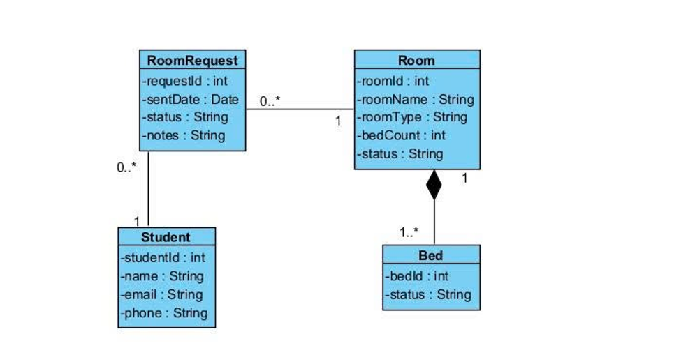
\includegraphics[width=0.72\textwidth]{assets/image4.png}
\caption{Sơ đồ lớp phân tích UC03 -- Sinh viên gửi yêu cầu đặt phòng}
\label{fig:uc03-class}
\end{figure}

\subsection{UC04 Cán bộ giữ phòng và giường cho sinh viên}

\subsubsection{Mục đích và mô tả chức năng}

\paragraph{Mục đích:}

Chức năng cho phép cán bộ xử lý yêu cầu đặt phòng của sinh viên bằng cách giữ một giường cụ thể cho sinh viên đó, hoặc từ chối yêu cầu khi không đáp ứng điều kiện. Dữ liệu giữ chỗ là đầu vào cho việc lập hợp đồng ở UC05.

\paragraph{Mô tả:}

Cán bộ xem danh sách yêu cầu đang chờ xử lý, chọn một yêu cầu và chọn giường cụ thể trong phòng phù hợp. Trước khi xác nhận, hệ thống kiểm tra lại trạng thái giường và xung đột thời gian để không giường nào bị giữ cho nhiều sinh viên. Khi thành công, hệ thống tạo bản ghi giữ chỗ, chuyển giường từ \textbf{trống} sang \textbf{đang giữ} và chuyển yêu cầu sang \textbf{Đã giữ chỗ}.

Để hạn chế hai yêu cầu đồng thời cùng giữ một giường, hệ thống có thể dùng khóa tạm có thời hạn trong Redis. Kết quả cuối cùng vẫn phải được kiểm tra và ghi nhận bằng giao dịch trong PostgreSQL.

\subsubsection{Tác nhân, tiền điều kiện và hậu điều kiện}

\begin{table}[H]
\centering
\small
\caption{Tác nhân, tiền điều kiện và hậu điều kiện của UC04}
\label{tab:ch2-7}
\begin{tabularx}{\textwidth}{|>{\raggedright\arraybackslash}p{0.32\textwidth}|>{\raggedright\arraybackslash}X|}
\hline
\textbf{Mục} & \textbf{Nội dung} \\
\hline
\textbf{Use Case ID} & UC04 \\
\hline
\textbf{Tên Use Case} & Cán bộ giữ phòng và giường cho sinh viên \\
\hline
\textbf{Tác nhân chính} & Cán bộ quản lý ký túc xá \\
\hline
\textbf{Tác nhân phụ} & Không có tác nhân trực tiếp \\
\hline
\textbf{Tiền điều kiện} & Cán bộ đã đăng nhập và có quyền xử lý yêu cầu đặt phòng. Có ít nhất một yêu cầu ở trạng thái "Chờ xử lý". Phòng và giường liên quan đã tồn tại trong hệ thống. \\
\hline
\textbf{Hậu điều kiện thành công} & \textit{Trường hợp giữ chỗ:} một bản ghi giữ chỗ được tạo, gắn yêu cầu, sinh viên và giường; giường chuyển sang "đang giữ"; yêu cầu chuyển sang "Đã giữ chỗ". \textit{Trường hợp từ chối:} yêu cầu chuyển sang "Bị từ chối" kèm lý do; giường không thay đổi. \\
\hline
\textbf{Hậu điều kiện thất bại} & Không tạo bản ghi giữ chỗ; trạng thái giường và yêu cầu giữ nguyên như trước thao tác; khóa tạm (nếu đã tạo) được giải phóng. \\
\hline
\end{tabularx}
\end{table}

\subsubsection{Luồng sự kiện chính}

\begin{enumerate}[leftmargin=1.6em]
\item Cán bộ chọn chức năng \textbf{"Giữ phòng và giường"}.
\item Hệ thống hiển thị danh sách yêu cầu đặt phòng ở trạng thái "Chờ xử lý".
\item Cán bộ chọn một yêu cầu cần xử lý.
\item Hệ thống hiển thị thông tin yêu cầu (sinh viên, phòng đề nghị, ngày dự kiến bắt đầu, ghi chú) và danh sách giường đang trống của phòng.
\item Cán bộ chọn một giường cụ thể để giữ cho sinh viên.
\item Cán bộ chọn \textbf{"Xác nhận giữ chỗ"}.
\item Hệ thống kiểm tra lại tại thời điểm xử lý:
\begin{itemize}
\item Yêu cầu vẫn ở trạng thái "Chờ xử lý".
\item Giường vẫn ở trạng thái trống và chưa có khóa giữ hợp lệ.
\item Giường không xung đột thời gian với giữ chỗ hoặc hợp đồng khác.
\item Sinh viên không có hợp đồng lưu trú đang hiệu lực.
\end{itemize}
\item Hệ thống tạo khóa giữ giường có thời hạn cho giường được chọn.
\item Hệ thống mở giao dịch cơ sở dữ liệu và thực hiện đồng thời:
\begin{itemize}
\item Tạo bản ghi giữ chỗ (yêu cầu, sinh viên, giường, cán bộ, thời điểm giữ, thời hạn giữ).
\item Cập nhật trạng thái giường từ \textbf{trống} sang \textbf{đang giữ}.
\item Cập nhật trạng thái yêu cầu sang \textbf{Đã giữ chỗ}.
\end{itemize}
\item Hệ thống hoàn tất giao dịch và làm mới dữ liệu tìm phòng đã lưu tạm liên quan.
\item Hệ thống thông báo \textbf{"Giữ chỗ thành công"} cho cán bộ; sinh viên xem được kết quả xử lý yêu cầu của mình.
\end{enumerate}

\subsubsection{Luồng thay thế và ngoại lệ}

\paragraph{Luồng thay thế}

\begin{itemize}[leftmargin=1.4em]
\item 3a. Cán bộ từ chối yêu cầu: Cán bộ chọn "Từ chối" và nhập lý do. Hệ thống chuyển yêu cầu sang "Bị từ chối", lưu lý do và không thay đổi dữ liệu giường. Sinh viên xem được kết quả và lý do.
\item 3b. Cán bộ không tiếp tục xử lý: Cán bộ hủy thao tác. Hệ thống quay lại danh sách yêu cầu chờ xử lý và không thay đổi dữ liệu.
\item 4a. Phòng đề nghị không còn giường trống: Hệ thống thông báo cho cán bộ. Cán bộ có thể chọn phòng khác còn chỗ phù hợp hoặc từ chối yêu cầu.
\item 7a. Yêu cầu không còn ở trạng thái chờ xử lý: Hệ thống dừng thao tác, thông báo yêu cầu đã được xử lý và tải lại danh sách.
\item 7b. Giường đã bị giữ hoặc đang thuê: Nếu giường đã có khóa giữ hợp lệ hoặc không còn trống (do cán bộ khác vừa xử lý), hệ thống từ chối và yêu cầu cán bộ chọn giường khác.
\item 7c. Sinh viên đã có hợp đồng đang hiệu lực: Hệ thống không cho giữ chỗ và gợi ý cán bộ từ chối yêu cầu.
\item Luồng ngoại lệ
\item 8a. Redis không khả dụng: Hệ thống không xác nhận giữ chỗ chỉ dựa trên dữ liệu tạm. Hệ thống vẫn kiểm tra và khóa dữ liệu ngay trong giao dịch PostgreSQL rồi mới xác nhận (BR12).
\item 9a. Lỗi khi ghi dữ liệu: Hệ thống hủy toàn bộ giao dịch, không tạo bản ghi giữ chỗ, giữ nguyên trạng thái giường và yêu cầu, giải phóng khóa tạm và thông báo lỗi cho cán bộ.
\item 9b. Xung đột đồng thời khi lưu: Nếu giao dịch phát hiện giường vừa bị thay đổi bởi yêu cầu khác, hệ thống hủy giao dịch và thông báo cán bộ chọn lại giường.
\end{itemize}

\subsubsection{Quy tắc nghiệp vụ và dữ liệu liên quan}

\paragraph{Quy tắc nghiệp vụ}

\begin{itemize}[leftmargin=1.4em]
\item BR03: Giường chỉ ở một trạng thái tại một thời điểm.
\item BR04: Một giường không được giữ hoặc phân cho nhiều sinh viên cùng lúc.
\item BR12: Trước khi giữ giường, hệ thống phải kiểm tra lại trạng thái tại thời điểm xử lý, không dùng dữ liệu cũ.
\item BR-UC04-01: Chỉ giữ chỗ cho yêu cầu ở trạng thái "Chờ xử lý".
\item BR-UC04-02: Chỉ giữ giường đang ở trạng thái trống; sau khi giữ, giường chuyển sang "đang giữ".
\item BR-UC04-03: Một yêu cầu chỉ được giữ tối đa một giường; một sinh viên chỉ có một giữ chỗ hợp lệ tại một thời điểm.
\item BR-UC04-04: Việc tạo giữ chỗ, cập nhật giường và cập nhật yêu cầu được thực hiện trong cùng một giao dịch: hoặc hoàn tất toàn bộ, hoặc không thay đổi gì.
\item BR-UC04-05: Giữ chỗ có thời hạn. Nếu quá thời hạn mà chưa lập hợp đồng (UC05), giữ chỗ hết hiệu lực và giường quay về trạng thái trống.
\item BR-UC04-06: Redis chỉ hỗ trợ khóa giữ tạm và tăng tốc; nếu Redis lỗi, tính đúng đắn vẫn dựa vào PostgreSQL.
\item BR-UC04-07: Khi từ chối yêu cầu, cán bộ phải nhập lý do.
\item Dữ liệu liên quan
\end{itemize}

\begin{table}[H]
\centering
\small
\caption{Các đối tượng dữ liệu liên quan đến UC04}
\label{tab:ch2-8}
\begin{tabularx}{\textwidth}{|>{\raggedright\arraybackslash}p{0.28\textwidth}|>{\raggedright\arraybackslash}X|>{\raggedright\arraybackslash}p{0.28\textwidth}|}
\hline
\textbf{Đối tượng} & \textbf{Thuộc tính chính} & \textbf{Vai trò trong UC} \\
\hline
Yêu cầu đặt phòng (BookingRequest) & requestId, studentId, roomId, status, rejectReason & Được đọc và cập nhật trạng thái \\
\hline
Giữ chỗ (Reservation) & reservationId, requestId, studentId, bedId, staffId, reservedAt, expiresAt, status & Được tạo mới; là căn cứ lập hợp đồng ở UC05 \\
\hline
Giường (Bed) & bedId, roomId, status & Được kiểm tra và chuyển từ "trống" sang "đang giữ" \\
\hline
Phòng (Room) & roomId, building, roomType, fee & Cung cấp thông tin và danh sách giường \\
\hline
Sinh viên (Student) & studentId, họ tên & Người được giữ chỗ \\
\hline
Cán bộ (Staff) & staffId, họ tên & Người thực hiện giữ chỗ \\
\hline
Hợp đồng (Contract) & contractId, studentId, status & Chỉ đọc, dùng để kiểm tra BR06 \\
\hline
\end{tabularx}
\end{table}

\section{Phân tích nhóm chức năng thuê phòng}

\subsection{UC05 Cán bộ lập hợp đồng thuê phòng cho sinh viên}

\subsubsection{Mục đích và mô tả chức năng}

Mục đích:

Chức năng cho phép cán bộ quản lý ký túc xá lập hợp đồng thuê phòng cho sinh viên sau khi sinh viên đã được giữ một chỗ ở hợp lệ. Hợp đồng là cơ sở ghi nhận chính thức thông tin về sinh viên, phòng, giường, thời hạn lưu trú và mức phí áp dụng, đồng thời là đầu vào cho nghiệp vụ bàn giao phòng ở UC06.

Mô tả:

Sau khi sinh viên có một giường được giữ hợp lệ từ giai đoạn đặt phòng, cán bộ lựa chọn sinh viên cần lập hợp đồng. Hệ thống kiểm tra lại thông tin giữ chỗ, trạng thái hiện tại của giường và tình trạng hợp đồng của sinh viên. Nếu các điều kiện được đáp ứng, cán bộ nhập hoặc xác nhận các thông tin về thời hạn hợp đồng và mức phí. Hệ thống sau đó tạo và lưu hợp đồng.

Việc lập hợp đồng tại UC05 chưa đồng nghĩa sinh viên đã chính thức nhận phòng. Hợp đồng chỉ chuyển sang trạng thái có hiệu lực và giường chỉ chuyển sang trạng thái đang thuê sau khi cán bộ hoàn thành việc bàn giao phòng tại UC06

\subsubsection{Tác nhân, tiền điều kiện và hậu điều kiện}

\begin{table}[H]
\centering
\small
\caption{Tác nhân, tiền điều kiện và hậu điều kiện của UC05}
\label{tab:ch2-9}
\begin{tabularx}{\textwidth}{|>{\raggedright\arraybackslash}p{0.32\textwidth}|>{\raggedright\arraybackslash}X|}
\hline
\textbf{Mục} & \textbf{Nội dung} \\
\hline
\textbf{Use Case ID} & UC05 \\
\hline
\textbf{Tên Use Case} & Cán bộ lập hợp đồng thuê phòng cho sinh viên \\
\hline
\textbf{Tác nhân chính} & Cán bộ quản lý ký túc xá \\
\hline
\textbf{Tác nhân phụ} & Không có tác nhân trực tiếp \\
\hline
\textbf{Tiền điều kiện} & Cán bộ đã đăng nhập và có quyền thực hiện chức năng lập hợp đồng. Sinh viên đã có một chỗ được giữ hợp lệ. Thông tin sinh viên, phòng và giường đã tồn tại trong hệ thống. \\
\hline
\textbf{Hậu điều kiện thành công} & Một hợp đồng lưu trú mới được tạo và lưu, gắn với sinh viên, phòng và giường đã được giữ. Hợp đồng ghi nhận thời gian bắt đầu, thời gian kết thúc, mức phí và trạng thái. Hợp đồng chưa chuyển sang trạng thái có hiệu lực cho đến khi bàn giao phòng thành công. \\
\hline
\textbf{Hậu điều kiện thất bại} & Không có hợp đồng mới được tạo; dữ liệu giữ chỗ, giường và các dữ liệu liên quan không bị thay đổi. \\
\hline
\end{tabularx}
\end{table}

\subsubsection{Luồng sự kiện chính}

\begin{enumerate}[leftmargin=1.6em]
\item Cán bộ chọn chức năng \textbf{“Lập hợp đồng thuê phòng”}.
\item Hệ thống hiển thị danh sách các sinh viên đã có chỗ được giữ hợp lệ và đủ điều kiện để lập hợp đồng.
\item Cán bộ lựa chọn sinh viên cần lập hợp đồng.
\item Hệ thống lấy thông tin giữ chỗ tương ứng và kiểm tra lại trạng thái hiện tại của sinh viên và giường.
\item Hệ thống kiểm tra:
\end{enumerate}

\begin{itemize}[leftmargin=1.4em]
\item Sinh viên có chỗ được giữ hợp lệ.
\item Giường vẫn đang được giữ cho đúng sinh viên.
\item Sinh viên không có hợp đồng lưu trú khác đang có hiệu lực.
\end{itemize}

\begin{enumerate}[leftmargin=1.6em]
\item Nếu các điều kiện được đáp ứng, hệ thống hiển thị thông tin lập hợp đồng gồm:
\end{enumerate}

\begin{itemize}[leftmargin=1.4em]
\item Thông tin sinh viên.
\item Thông tin phòng.
\item Thông tin giường.
\item Thời gian bắt đầu hợp đồng.
\item Thời gian kết thúc hợp đồng.
\item Mức phí áp dụng.
\end{itemize}

\begin{enumerate}[leftmargin=1.6em]
\item Cán bộ nhập hoặc xác nhận các thông tin của hợp đồng.
\item Cán bộ chọn \textbf{“Lập hợp đồng”}.
\item Hệ thống kiểm tra tính đầy đủ và hợp lệ của dữ liệu được nhập.
\item Hệ thống tạo bản ghi hợp đồng lưu trú, liên kết với sinh viên và chỗ ở đã được giữ.
\item Hệ thống lưu hợp đồng nhưng chưa chuyển hợp đồng sang trạng thái có hiệu lực.
\item Hệ thống thông báo \textbf{“Lập hợp đồng thành công”} cho cán bộ. Hợp đồng sau đó có thể được sử dụng trong UC06 – Cán bộ xác nhận bàn giao phòng cho sinh viên.
\end{enumerate}

\paragraph{d.Luồng thay thế}

\begin{itemize}[leftmargin=1.4em]
\item 3a. Cán bộ không tiếp tục lập hợp đồng:
\end{itemize}

Cán bộ hủy thao tác. Hệ thống quay lại danh sách sinh viên/chỗ đã được giữ và không tạo hợp đồng.

\begin{itemize}[leftmargin=1.4em]
\item 4a. Thông tin giữ chỗ không còn hợp lệ:
\end{itemize}

Hệ thống không cho phép tiếp tục lập hợp đồng và yêu cầu cán bộ kiểm tra lại thông tin giữ chỗ.

\begin{itemize}[leftmargin=1.4em]
\item 5a. Giường không còn ở trạng thái phù hợp:
\end{itemize}

Nếu tại thời điểm kiểm tra, giường không còn được giữ hợp lệ cho sinh viên đang được chọn, hệ thống dừng quá trình lập hợp đồng và thông báo cho cán bộ.

\begin{itemize}[leftmargin=1.4em]
\item 5b. Sinh viên đã có hợp đồng đang có hiệu lực:
\end{itemize}

Hệ thống từ chối lập hợp đồng mới và thông báo sinh viên đang có hợp đồng lưu trú còn hiệu lực.

\paragraph{e.Luồng ngoại lệ}

\begin{itemize}[leftmargin=1.4em]
\item 9a. Dữ liệu hợp đồng thiếu hoặc không hợp lệ:
\end{itemize}

Hệ thống hiển thị thông tin lỗi tại trường tương ứng và yêu cầu cán bộ kiểm tra, chỉnh sửa trước khi tiếp tục.

\begin{itemize}[leftmargin=1.4em]
\item 10a. Có thay đổi trạng thái dữ liệu trong quá trình xử lý:
\end{itemize}

Hệ thống kiểm tra lại trạng thái giường và dữ liệu giữ chỗ trước khi lưu. Nếu điều kiện không còn được đáp ứng, hợp đồng không được tạo.

\begin{itemize}[leftmargin=1.4em]
\item 11a. Lỗi khi lưu dữ liệu:
\end{itemize}

Hệ thống không ghi nhận hợp đồng mới, giữ nguyên dữ liệu trước khi thực hiện thao tác và thông báo lỗi cho cán bộ.

Cách xử lý này phù hợp với yêu cầu chung của hệ thống là phải kiểm soát trạng thái để tránh việc một giường bị phân cho nhiều sinh viên

\subsubsection{Quy tắc nghiệp vụ và dữ liệu liên quan}


\subsubsection{Sơ đồ lớp UC05}


\subsection{UC06 Cán bộ xác nhận bàn giao phòng cho sinh viên}

\subsubsection{Mục đích và mô tả chức năng}

\paragraph{Mục đích:}

Chức năng cho phép cán bộ quản lý ký túc xá xác nhận việc bàn giao chỗ ở cho sinh viên sau khi hợp đồng thuê phòng đã được lập. Việc xác nhận bàn giao đánh dấu thời điểm sinh viên chính thức nhận và được quyền sử dụng giường đã được phân.

\paragraph{Mô tả:}

Sau khi UC05 hoàn tất việc lập hợp đồng, cán bộ lựa chọn hợp đồng cần thực hiện bàn giao. Hệ thống kiểm tra tính hợp lệ của hợp đồng và tình trạng hiện tại của giường. Nếu các điều kiện được đáp ứng, cán bộ xác nhận sinh viên đã nhận chỗ ở.

Khi bàn giao thành công, hệ thống ghi nhận thông tin bàn giao, chuyển hợp đồng sang trạng thái \textbf{có hiệu lực} và cập nhật trạng thái giường từ \textbf{đang giữ} sang \textbf{đang thuê}.

\subsubsection{Tác nhân, tiền điều kiện và hậu điều kiện}

\begin{table}[H]
\centering
\small
\caption{Tác nhân, tiền điều kiện và hậu điều kiện của UC06}
\label{tab:ch2-10}
\begin{tabularx}{\textwidth}{|>{\raggedright\arraybackslash}p{0.32\textwidth}|>{\raggedright\arraybackslash}X|}
\hline
\textbf{Mục} & \textbf{Nội dung} \\
\hline
\textbf{Use Case ID} & UC06 \\
\hline
\textbf{Tên Use Case} & Cán bộ xác nhận bàn giao phòng cho sinh viên \\
\hline
\textbf{Tác nhân chính} & Cán bộ quản lý ký túc xá \\
\hline
\textbf{Tác nhân phụ} & Không có tác nhân trực tiếp \\
\hline
\textbf{Tiền điều kiện} & Cán bộ đã đăng nhập và có quyền thực hiện chức năng bàn giao. Sinh viên đã có hợp đồng thuê phòng được lập hợp lệ. Giường liên kết với hợp đồng vẫn đang được giữ cho sinh viên và chưa được phân cho người khác. \\
\hline
\textbf{Hậu điều kiện thành công} & Thông tin bàn giao được ghi nhận; hợp đồng chuyển sang trạng thái có hiệu lực; giường chuyển từ trạng thái đang giữ sang đang thuê. \\
\hline
\textbf{Hậu điều kiện thất bại} & Không ghi nhận bàn giao; hợp đồng và trạng thái giường giữ nguyên trạng thái trước khi thực hiện thao tác. \\
\hline
\end{tabularx}
\end{table}

\subsubsection{Luồng sự kiện chính}

Cán bộ chọn chức năng \textbf{“Xác nhận bàn giao phòng”}.

Hệ thống hiển thị các hợp đồng đã được lập và đang chờ thực hiện bàn giao.

Cán bộ lựa chọn hợp đồng của sinh viên cần bàn giao phòng.

Hệ thống hiển thị các thông tin liên quan gồm:

\begin{itemize}[leftmargin=1.4em]
\item Thông tin sinh viên.
\item Thông tin hợp đồng.
\item Phòng được phân.
\item Giường được phân.
\item Thời gian của hợp đồng.
\item Mức phí áp dụng.
\item Trạng thái hiện tại của hợp đồng và giường.
\end{itemize}

Hệ thống kiểm tra điều kiện bàn giao:

\begin{itemize}[leftmargin=1.4em]
\item Hợp đồng tồn tại và hợp lệ.
\item Hợp đồng chưa được bàn giao trước đó.
\item Giường vẫn đang được giữ cho đúng sinh viên.
\item Sinh viên không có hợp đồng lưu trú khác đang có hiệu lực.
\item Giường chưa được phân cho sinh viên khác.
\end{itemize}

Khi các điều kiện được đáp ứng, hệ thống cho phép cán bộ thực hiện xác nhận bàn giao.

Cán bộ chọn \textbf{“Xác nhận bàn giao”}.

Hệ thống ghi nhận thông tin bàn giao phòng.

Hệ thống cập nhật trạng thái hợp đồng sang \textbf{có hiệu lực}.

Hệ thống cập nhật trạng thái giường từ \textbf{đang giữ} sang \textbf{đang thuê}.

Hệ thống lưu toàn bộ thay đổi.

Hệ thống thông báo \textbf{“Bàn giao phòng thành công”} cho cán bộ.

\subsubsection{Luồng thay thế}

\paragraph{3a. Cán bộ không tiếp tục bàn giao}

Cán bộ hủy thao tác. Hệ thống quay trở lại danh sách hợp đồng chờ bàn giao và không thay đổi dữ liệu.

\paragraph{5a. Hợp đồng không còn hợp lệ}

Nếu hợp đồng không tồn tại hoặc không còn ở trạng thái phù hợp để bàn giao, hệ thống từ chối thao tác và thông báo cho cán bộ kiểm tra lại hợp đồng.

\paragraph{5b. Hợp đồng đã được bàn giao trước đó}

Nếu hợp đồng đã có hiệu lực do quá trình bàn giao đã được thực hiện, hệ thống không cho phép xác nhận bàn giao lần nữa.

\paragraph{5c. Giường không còn được giữ cho sinh viên}

Nếu tại thời điểm xử lý, trạng thái giường không còn phù hợp hoặc giường không còn gắn với đúng sinh viên trong hợp đồng, hệ thống dừng quá trình bàn giao và thông báo cho cán bộ.

\paragraph{5d. Sinh viên đã có hợp đồng khác đang có hiệu lực}

Hệ thống không cho phép bàn giao hợp đồng mới để tránh một sinh viên đồng thời có nhiều hợp đồng lưu trú còn hiệu lực.

\subsubsection{Luồng ngoại lệ}

\paragraph{8a. Không thể ghi nhận thông tin bàn giao}

Nếu xảy ra lỗi khi tạo dữ liệu bàn giao, hệ thống không thực hiện cập nhật trạng thái hợp đồng và giường.

\paragraph{9a. Cập nhật hợp đồng thất bại}

Nếu không thể chuyển hợp đồng sang trạng thái có hiệu lực, toàn bộ thao tác bàn giao bị hủy.

\paragraph{10a. Cập nhật trạng thái giường thất bại}

Nếu hợp đồng đã được xử lý nhưng không thể cập nhật giường sang trạng thái đang thuê, hệ thống phải hủy toàn bộ thay đổi để không tạo ra trạng thái dữ liệu không nhất quán.

\subsubsection{Quy tắc nghiệp vụ và dữ liệu liên quan}


\subsubsection{Sơ đồ lớp UC06}


\section{Phân tích nhóm chức năng đóng phí}

\subsection{UC07 Hệ thống lập khoản phí nội trú cho sinh viên}

\subsubsection{Mục đích và mô tả chức năng}

Mục đích: tự động lập các khoản phí nội trú theo từng kỳ cho sinh viên đang ở KTX, để sinh viên có căn cứ thanh toán (UC08).

Mô tả: đến kỳ thu phí, cán bộ kích hoạt chức năng. Hệ thống lấy các hợp đồng còn hiệu lực, tính số tiền theo phí phòng, tạo bản ghi DormitoryFee với trạng thái "Chưa thanh toán" và thông báo cho sinh viên.

\subsubsection{Tác nhân, tiền điều kiện và hậu điều kiện}

Tác nhân chính : Cán bộ quản lý ký túc xá

Tác nhân phụ: Không có

Tiền điều kiện: Cán bộ đã đăng nhập vào hệ thống và có quyền quản lý tài chính/khoản phí. Dữ liệu danh mục kỳ thu, loại phí đã được thiết lập. Tồn tại ít nhất một hợp đồng thuê phòng đang có hiệu lực (ACTIVE) trong kỳ thu tương ứng.

Hậu điều kiện thành công: Các bản ghi khoản phí nội trú mới được tạo và lưu vào cơ sở dữ liệu với trạng thái "Chưa thanh toán". Sinh viên có thể tra cứu thấy khoản nợ phát sinh của mình trên hệ thống.

Hậu điều kiện thất bại: Không có khoản phí nào được tạo hoặc dữ liệu bị hủy toàn bộ nếu có lỗi giao dịch; thông tin công nợ giữ nguyên trạng thái trước đó.

\subsubsection{Luồng sự kiện chính}

Cán bộ chọn chức năng "Phát hành khoản phí nội trú theo kỳ".

Hệ thống hiển thị biểu mẫu chọn kỳ thu, loại phí và hạn nộp tiền.

Cán bộ chọn kỳ thu cần tính phí, nhập hạn nộp và chọn "Kiểm tra danh sách hợp đồng".

Hệ thống quét cơ sở dữ liệu, lọc các hợp đồng đang có hiệu lực (ACTIVE) và kiểm tra điều kiện phát sinh phí (chưa được lập phí cho kỳ này).

Hệ thống hiển thị danh sách dự kiến các khoản phí (Mã SV, họ tên, mã hợp đồng, phòng, số tiền theo tháng/kỳ, hạn nộp) để cán bộ đối chiếu.

Cán bộ kiểm tra danh sách và chọn "Xác nhận phát hành phí".

Hệ thống mở giao dịch cơ sở dữ liệu (PostgreSQL Transaction):

\begin{itemize}[leftmargin=1.4em]
\item Tạo các bản ghi Fee tương ứng với từng hợp đồng.
\item Thiết lập trạng thái khoản phí là UNPAID ("Chưa thanh toán").
\item Ghi nhận ngày tạo, hạn thanh toán và cán bộ thực hiện.
\end{itemize}

Hệ thống hoàn tất giao dịch cơ sở dữ liệu.

Hệ thống gửi thông báo khoản phí mới vào trang quản lý của các sinh viên liên quan.

Hệ thống hiển thị thông báo "Phát hành khoản phí nội trú thành công" kèm tổng số lượng bản ghi đã tạo.

\subsubsection{Luồng thay thế và ngoại lệ}

\paragraph{Luồng thay thế:}

\begin{itemize}[leftmargin=1.4em]
\item 3a. Cán bộ hủy thao tác: Cán bộ chọn hủy; hệ thống quay trở lại màn hình quản trị tài chính, không lưu dữ liệu.
\item 4a. Không tìm thấy hợp đồng đủ điều kiện: Hệ thống thông báo không có hợp đồng đang hiệu lực hoặc các hợp đồng đã được tạo phí cho kỳ này, dừng quá trình phát hành.
\item 6a. Cán bộ điều chỉnh danh sách: Cán bộ có thể bỏ chọn một số sinh viên có trường hợp đặc biệt (ví dụ miễn giảm) trước khi phát hành hàng loạt.
\item Luồng ngoại lệ:
\item 2a. Hạn thanh toán không hợp lệ: Nếu cán bộ nhập hạn thanh toán nhỏ hơn hoặc bằng ngày phát hành, hệ thống báo lỗi và yêu cầu chọn lại.
\item 7a. Lỗi ghi dữ liệu/xung đột giao dịch: Hệ thống rollback toàn bộ giao dịch, không tạo khoản phí dở dang và báo lỗi cho cán bộ.
\end{itemize}

\subsubsection{Quy tắc nghiệp vụ và dữ liệu liên quan}

Quy tắc nghiệp vụ:

\begin{itemize}[leftmargin=1.4em]
\item BR01, BR02: Chỉ cán bộ quản lý mới có quyền phát hành khoản phí.
\item BR08: Chỉ phát sinh và phát hành khoản phí cho các hợp đồng đang có hiệu lực (status = ACTIVE).
\item BR-UC07-01: Mỗi hợp đồng chỉ được phát hành một khoản phí nội trú duy nhất cho mỗi kỳ.
\item BR-UC07-02: Hạn nộp phí phải sau thời điểm phát hành.
\item BR-UC07-03: Toàn bộ các bản ghi phí trong đợt phát hành phải được tạo trong cùng một giao dịch toàn vẹn (ACID).
\end{itemize}

Dữ liệu liên quan:

\subsubsection{Sơ đồ lớp UC07}


\subsection{UC08 Sinh viên thanh toán khoản phí nội trú}

\subsubsection{a Mục đích và mô tả chức năng}

Mục đích: Cho phép sinh viên tra cứu công nợ cá nhân và thực hiện thanh toán các khoản phí nội trú đang ở trạng thái chưa thanh toán.

Mô tả: Sinh viên đăng nhập vào hệ thống, xem danh sách các khoản phí nội trú của mình, chọn khoản phí cần thanh toán và chọn phương thức thanh toán. Hệ thống kiểm tra tính hợp lệ của khoản phí, mô phỏng/ghi nhận kết quả giao dịch thanh toán (Payment Transaction), cập nhật trạng thái khoản phí sang "Đã thanh toán" và lưu biên lai giao dịch.

\subsubsection{Tác nhân, tiền điều kiện và hậu điều kiện}

Tác nhân chính: Sinh viên

Tác nhân phụ: Cổng thanh toán / Hệ thống mô phỏng thanh toán

Tiền điều kiện: Sinh viên đã đăng nhập hệ thống. Tồn tại ít nhất một khoản phí của sinh viên có trạng thái "Chưa thanh toán" (status = UNPAID).

Hậu điều kiện thành công: Giao dịch thanh toán (PaymentTransaction) được tạo và lưu trữ. Khoản phí chuyển sang trạng thái "Đã thanh toán" (PAID). Sinh viên nhận được biên lai giao dịch thành công.

Hậu điều kiện thất bại: Giao dịch thất bại; trạng thái khoản phí vẫn là UNPAID; không ghi nhận biến động công nợ.

\subsubsection{Luồng sự kiện chính}

Sinh viên chọn chức năng "Khoản phí nội trú".

Hệ thống truy vấn và hiển thị danh sách các khoản phí của sinh viên (kỳ thu, số tiền, hạn nộp, trạng thái).

Sinh viên chọn một khoản phí đang ở trạng thái UNPAID và bấm "Thanh toán".

Hệ thống kiểm tra lại trạng thái khoản phí tại thời điểm thanh toán (đảm bảo vẫn là UNPAID và chưa bị khóa bởi giao dịch đang xử lý).

Hệ thống hiển thị màn hình xác nhận thanh toán (Mã khoản phí, tên sinh viên, số tiền cần đóng, phương thức thanh toán).

Sinh viên chọn phương thức thanh toán (ví dụ: chuyển khoản/mô phỏng cổng thanh toán) và chọn "Xác nhận thanh toán".

Hệ thống chuyển tiếp yêu cầu đến module xử lý/mô phỏng thanh toán.

Hệ thống nhận phản hồi thanh toán thành công.

Hệ thống mở giao dịch cơ sở dữ liệu:

\begin{itemize}[leftmargin=1.4em]
\item Tạo bản ghi giao dịch PaymentTransaction với mã giao dịch, số tiền, phương thức, thời gian thanh toán và kết quả SUCCESS.
\item Cập nhật trạng thái của bản ghi Fee từ UNPAID sang PAID.
\end{itemize}

Hệ thống lưu thành công giao dịch vào PostgreSQL.

Hệ thống hiển thị thông báo "Thanh toán thành công" và xuất biên lai thanh toán cho sinh viên.

\subsubsection{Luồng thay thế và ngoại lệ}

Luồng thay thế:

\begin{itemize}[leftmargin=1.4em]
\item 3a. Sinh viên hủy giao dịch: Sinh viên nhấn hủy tại bước xác nhận; hệ thống quay lại màn hình danh sách khoản phí, không thay đổi dữ liệu.
\item 4a. Khoản phí đã được thanh toán: Nếu khoản phí vừa được gạch nợ ở phiên khác, hệ thống thông báo "Khoản phí này đã được thanh toán" và tải lại danh sách.
\end{itemize}

Luồng ngoại lệ:

\begin{itemize}[leftmargin=1.4em]
\item 7a. Quá trình xử lý thanh toán bị từ chối / không thành công: Cổng thanh toán mô phỏng phản hồi giao dịch thất bại; hệ thống tạo bản ghi PaymentTransaction với trạng thái FAILED, giữ nguyên trạng thái UNPAID của khoản phí và hiển thị thông báo nguyên nhân thất bại cho sinh viên.
\item 9a. Lỗi cơ sở dữ liệu khi cập nhật: Hệ thống hủy giao dịch (rollback), trạng thái khoản phí không thay đổi và hiển thị cảnh báo để sinh viên đối soát.
\end{itemize}

\subsubsection{Quy tắc nghiệp vụ và dữ liệu liên quan}


\subsubsection{Sơ đồ lớp UC08}


\section{Phân tích nhóm chức năng trả phòng}

\subsection{UC09 Sinh viên gửi yêu cầu trả phòng}

\subsubsection{Mục đích và mô tả chức năng}

Mục đích:

Chức năng cho phép sinh viên đang lưu trú tại ký túc xá gửi yêu cầu trả phòng khi không còn nhu cầu tiếp tục sử dụng chỗ ở. Yêu cầu được ghi nhận trên hệ thống và là cơ sở để cán bộ quản lý thực hiện xác nhận hoàn tất trả phòng tại UC10

Mô tả:

Sinh viên đăng nhập vào hệ thống và lựa chọn chức năng gửi yêu cầu trả phòng. Hệ thống kiểm tra hợp đồng lưu trú đang có hiệu lực và hiển thị thông tin phòng, giường tương ứng.

Sinh viên nhập thời gian dự kiến trả phòng và các thông tin cần thiết, sau đó xác nhận gửi yêu cầu. Hệ thống kiểm tra tính hợp lệ của dữ liệu và lưu yêu cầu với trạng thái "Chờ xử lý".

Sau khi gửi thành công, sinh viên có thể theo dõi trạng thái yêu cầu. Việc gửi yêu cầu chưa làm thay đổi trạng thái hợp đồng hoặc giải phóng giường.

\subsubsection{Tác nhân, tiền điều kiện và hậu điều kiện}

\begin{table}[H]
\centering
\small
\caption{Tác nhân, tiền điều kiện và hậu điều kiện của UC09}
\label{tab:ch2-11}
\begin{tabularx}{\textwidth}{|>{\raggedright\arraybackslash}p{0.32\textwidth}|>{\raggedright\arraybackslash}X|}
\hline
\textbf{Mục} & \textbf{Nội dung} \\
\hline
\textbf{Use Case ID} & UC09 \\
\hline
\textbf{Tên Use Case} & Sinh viên gửi yêu cầu trả phòng \\
\hline
\textbf{Tác nhân chính} & Sinh viên \\
\hline
\textbf{Tác nhân phụ} & Không có \\
\hline
\textbf{Tiền điều kiện} & Sinh viên đã đăng nhập vào hệ thống và có hợp đồng lưu trú đang có hiệu lực. Thông tin phòng và giường tương ứng đã tồn tại trong hệ thống. \\
\hline
\textbf{Hậu điều kiện thành công} & Yêu cầu trả phòng được tạo và lưu với trạng thái "Chờ xử lý". Hệ thống ghi nhận thông tin sinh viên, hợp đồng và thời gian dự kiến trả phòng. \\
\hline
\textbf{Hậu điều kiện thất bại} & Không có yêu cầu trả phòng mới được tạo. Thông tin hợp đồng và trạng thái giường không thay đổi. \\
\hline
\end{tabularx}
\end{table}

\subsubsection{Luồng sự kiện chính}

Luồng sự kiện chính của UC09 được thực hiện như sau:

\begin{enumerate}[leftmargin=1.6em]
\item Sinh viên đăng nhập vào hệ thống và lựa chọn chức năng "Gửi yêu cầu trả phòng".
\item Hệ thống tìm kiếm và kiểm tra hợp đồng lưu trú đang có hiệu lực của sinh viên.
\item Hệ thống hiển thị thông tin hợp đồng, phòng và giường mà sinh viên đang sử dụng.
\item Sinh viên nhập thời gian dự kiến trả phòng và ghi chú nếu có.
\item Sinh viên kiểm tra thông tin và nhấn nút "Gửi yêu cầu".
\item Hệ thống kiểm tra tính đầy đủ, hợp lệ của thông tin và trạng thái hợp đồng tại thời điểm xử lý.
\item Nếu dữ liệu hợp lệ, hệ thống tạo bản ghi yêu cầu trả phòng, liên kết với sinh viên và hợp đồng tương ứng.
\item Hệ thống thiết lập trạng thái yêu cầu là "Chờ xử lý" và ghi nhận thời điểm gửi.
\item Hệ thống lưu thông tin yêu cầu trả phòng vào cơ sở dữ liệu.
\item Hệ thống hiển thị thông báo gửi yêu cầu thành công. Sinh viên có thể theo dõi trạng thái xử lý của yêu cầu.
\end{enumerate}

\subsubsection{Luồng thay thế và ngoại lệ}

\paragraph{Luồng thay thế:}

\begin{itemize}[leftmargin=1.4em]
\item 2a. Sinh viên không có hợp đồng đang hiệu lực: Hệ thống thông báo sinh viên không có hợp đồng hợp lệ và không cho phép gửi yêu cầu trả phòng.
\item 4a. Sinh viên không nhập ghi chú: Hệ thống cho phép tiếp tục thực hiện vì ghi chú là thông tin không bắt buộc.
\item 5a. Sinh viên hủy thao tác: Hệ thống quay lại màn hình quản lý hợp đồng và không tạo yêu cầu trả phòng.
\item Luồng ngoại lệ:
\item 1a. Phiên đăng nhập không hợp lệ: Hệ thống yêu cầu sinh viên đăng nhập lại trước khi tiếp tục thao tác.
\item 6a. Thông tin không hợp lệ: Hệ thống hiển thị thông báo lỗi và yêu cầu sinh viên chỉnh sửa thông tin.
\item 6b. Trạng thái hợp đồng thay đổi: Nếu hợp đồng không còn hiệu lực tại thời điểm xử lý, hệ thống từ chối tạo yêu cầu.
\item 9a. Lỗi lưu dữ liệu: Hệ thống thông báo lỗi, không tạo yêu cầu trả phòng và giữ nguyên dữ liệu hiện tại.
\end{itemize}

\subsubsection{Quy tắc nghiệp vụ và dữ liệu liên quan}


\subsubsection{Biểu đồ hoạt động UC09}


\subsection{UC10 Cán bộ xác nhận hoàn tất trả phòng}

\subsubsection{Mục đích và mô tả chức năng}


\subsubsection{Tác nhân, tiền điều kiện và hậu điều kiện}


\subsubsection{Luồng sự kiện chính}


\subsubsection{Luồng thay thế và ngoại lệ}


\subsubsection{Quy tắc nghiệp vụ và dữ liệu liên quan}


\subsubsection{Biểu đồ hoạt động UC10}


